\chapter{Evaluación Tercer Parcial}
\newpage
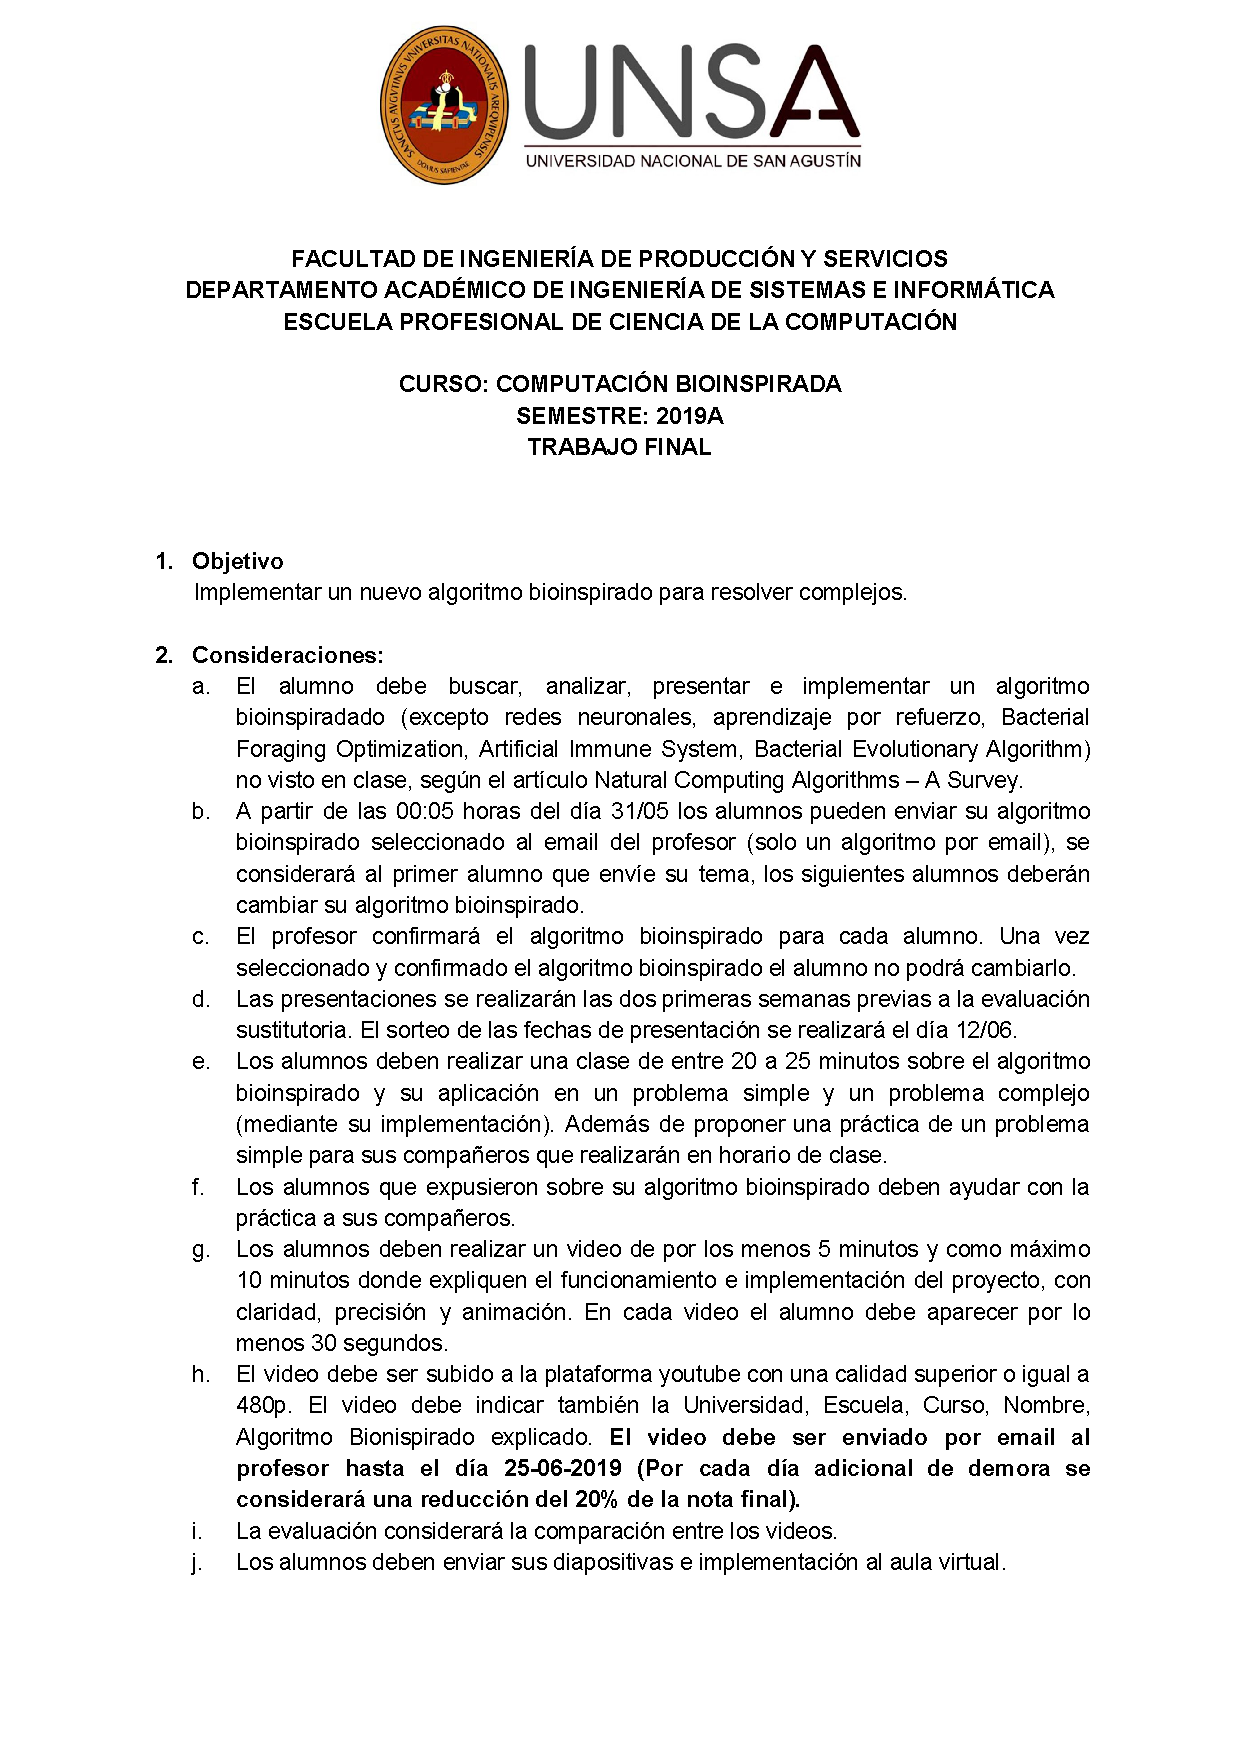
\includepdf[pages={1-}]{pdfs/prueba_3er_parcial.pdf}
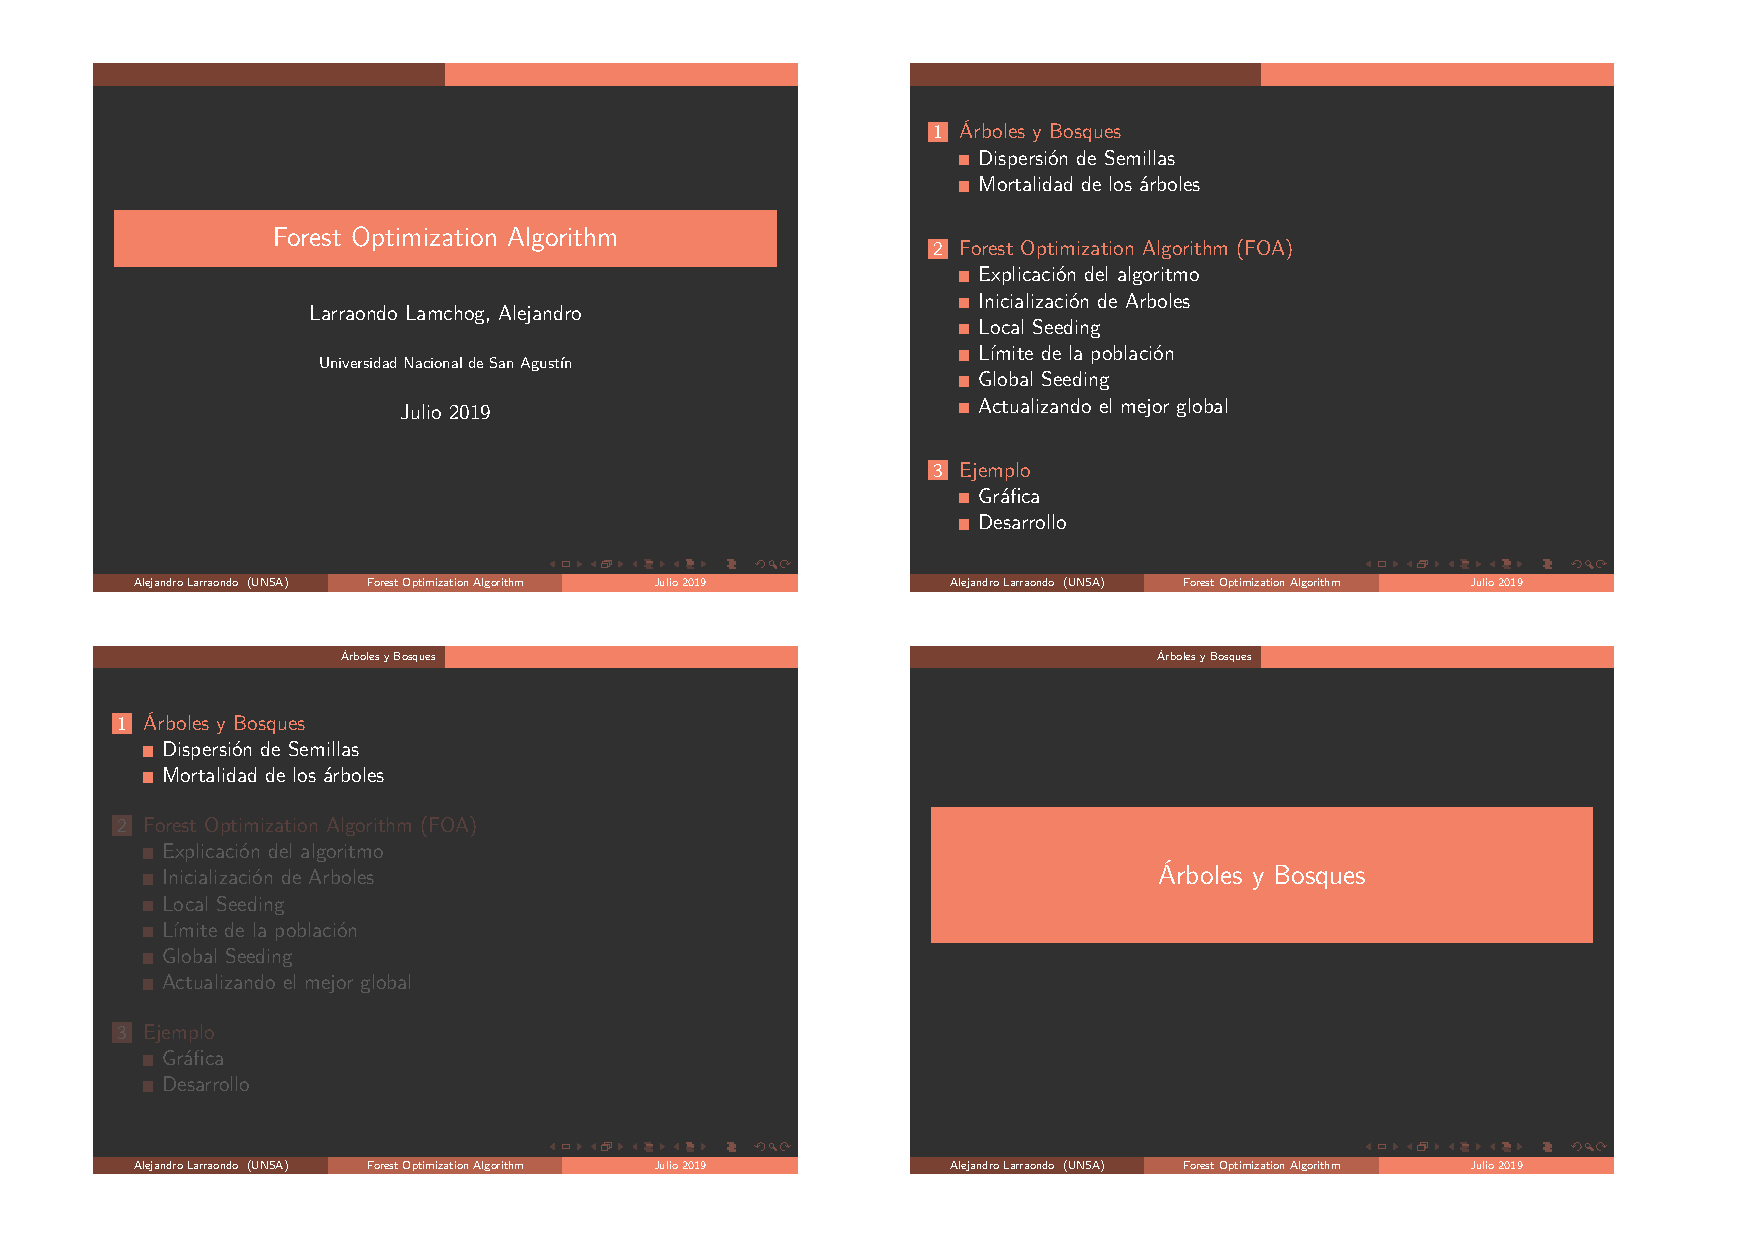
\includepdf[pages={1-}]{pdfs/prueba_3er_parcial_mejor_aprobada.pdf}
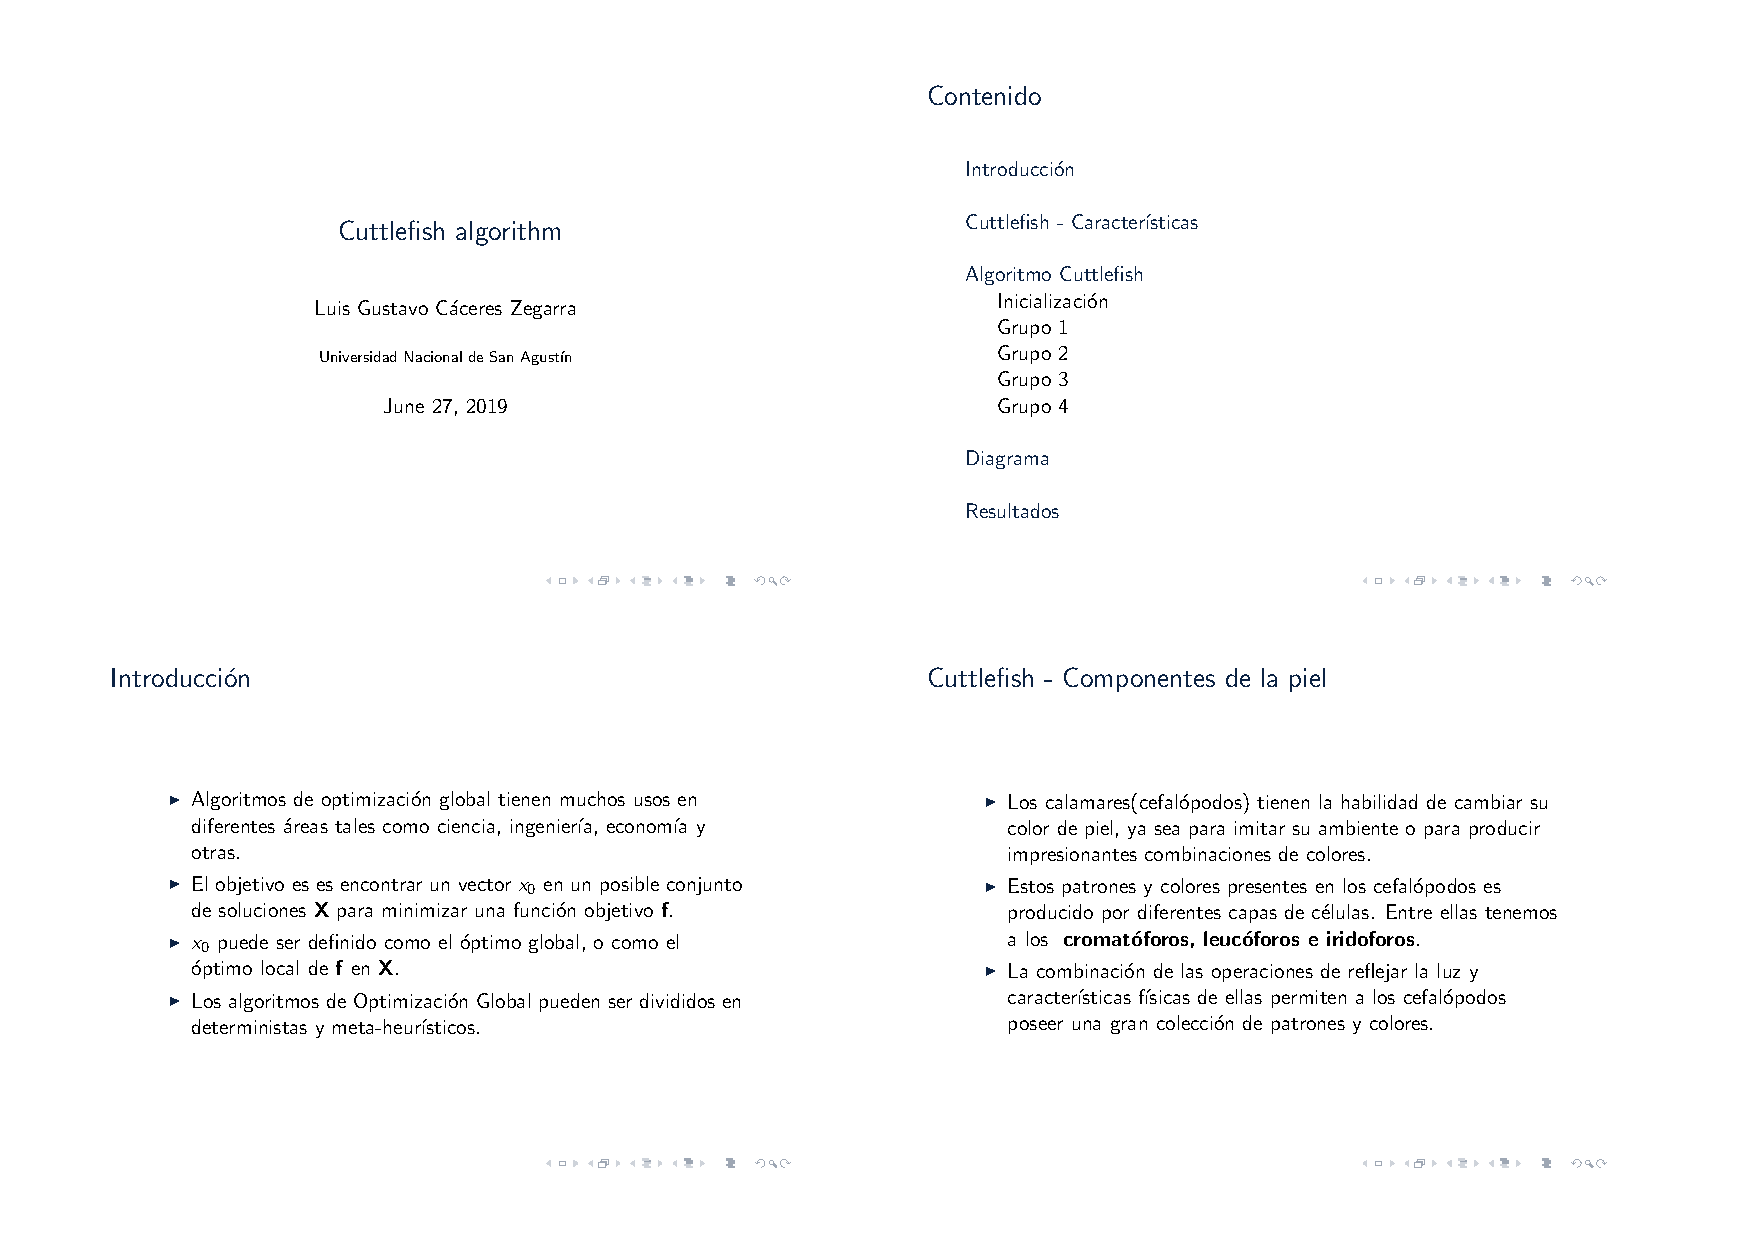
\includepdf[pages={1-}]{pdfs/prueba_3er_parcial_peor_aprobada.pdf}

\pagestyle{empty} % Disable headers and footers for the following pages

\section{Evidencias}
Rindieron la Tecera Evaluación Parcial (o Trabajo Final) 16 estudiantes de los 16 estudiantes matriculados, lo que representa un 100.0\%.

La nota promedio de los estudiantes que rindieron la Tercera Evaluación Parcial es 16.2 puntos. Las notas y la evidencia de la Tercera Evaluación Parcial se encuentran en la siguiente tabla:

\begin{table}[h]
\centering
\begin{tabular}{l|c|c}
\hline
\textbf{Apellidos y Nombres} & 
\textbf{Nota} & 
\textbf{Evidencia} 
\\ \hline
Amable Romero, Diego Javier &
17.0 &
\href{https://drive.google.com/open?id=1RGE-0KmemYyM1_d2kqPFSByuEEYTf70C}{Link}
\\ \hline
Bernal Chahuayo, Luis Antonio &
16.0 &
\href{https://drive.google.com/open?id=1FeRY8FPwENPs6JGo3LrUYZigr4FfQQH4}{Link}
\\ \hline
Caceres Zegarra, Luis Gustavo &
15.0 &
\href{https://drive.google.com/open?id=1aRhn2lBo3sZXlTMA4sh9wJ5r5g2bXE8T}{Link}
\\ \hline
Espinel Quispe, Ingrid Sally &
07.0 &
\href{https://drive.google.com/open?id=135na5wEvQ_LrngLGUhVwp92BpkZ2PblH}{Link}
\\ \hline
Gordillo Viña, Karen &
19.0 &
\href{https://drive.google.com/open?id=12-LqWuAXj5IB53-Me7gi4mJz6In7qewI}{Link}
\\ \hline
Gutierrez Salazar, Enrique Alonzo &
17.0 &
\href{https://drive.google.com/open?id=10fti0Nvn_GhppfJQ0cGxxPrEwGgbgulw}{Link}
\\ \hline
Hancco Tancayllo, Hermith &
15.0 &
\href{https://drive.google.com/open?id=15XyNJkvHo4XuC1ylerS8IQey5eImNxRR}{Link}
\\ \hline
Huaman Canqui Jair, Francesco &
16.0 &
\href{https://drive.google.com/open?id=1KHvPDBSUBZqywpxbN_niUf8PdkRjzBoC}{Link}
\\ \hline
Lacuaña Apaza, Margarita &
16.0 &
\href{https://drive.google.com/open?id=1OZAFwkOkPnFwLvVwAAH-jvAhziwBx09o}{Link}
\\ \hline
Larraondo Lancho, Alejandro Jesús &
19.0 &
\href{https://drive.google.com/open?id=1qjRtWRIrA7fcinCeWOX74rG9vonaawIF}{Link}
\\ \hline
Mamani Chirinos, Luis &
14.0 &
\href{https://drive.google.com/open?id=1JrGsIkJzS_lwTkOaSZdIipVaRmakLodP}{Link}
\\ \hline
Mendoza Villarroel, Alexis &
18.0 &
\href{https://drive.google.com/open?id=1xQ0p9bxbJRba3aqW5BiKMy3jFEyogEPM}{Link}
\\ \hline
Quincho Mamani, Lehi &
17.0 &
\href{https://drive.google.com/open?id=1X4sgTvGoHOD-xrGULO0eLx6MiX9UB26f}{Link}
\\ \hline
Quispe Quicano, Julio Cesar &
17.0 &
\href{https://drive.google.com/open?id=1498VuZAYY9B6AScuvHA5EMFrCAxscPer}{Link}
\\ \hline
Turpo Apaza, Crhistian Andrew &
17.0 &
\href{https://drive.google.com/open?id=14HnFWBEkh2y6LEVVtxKpaJqsddbscORE}{Link}
\\ \hline
Uñapilco Chambi, Katherin &
19.0 &
\href{https://drive.google.com/open?id=1fXM-Ufvhy0M0FVDEkZ8dclLG2OK0P8ga}{Link}
\\ \hline
\end{tabular}
\caption{Resultados Tercera Evaluación Parcial}
\label{tab:evalucion_parcial_3} % Unique label used for referencing the table in-text
%\addcontentsline{toc}{table}{Table \ref{tab:example}} % Uncomment to add the table to the table of contents
\end{table}
%------------------------------------------------

